\chapter{Macchina di Turing}
\section{Macchina di Turing}
La \textbf{macchina di Turing} consiste di un controllo finito che può trovarsi
in un stato, scelto in un insieme finito. Tale macchina è composta da un
\textbf{nastro}, potenzialmente infinito, diviso in \textbf{celle}, ognuna delle
quali può contenere un simbolo scelto in un insieme finito chiamato
\textbf{alfabeto}.

L'input è una stringa di lunghezza finita formata da simboli scelti
dall'\textit{alfabeto} di input ($\Sigma$), e viene inizialmente posto sul nastro.
In tutte le altre celle, che si estendono sia a destra che a sinistra senza limiti,
è presente il simbolo \textit{blank} ($\sqcup$), il quale specifica che in quella
posizione non è presente un simbolo dell'alfabeto. C'è però un eccezione, infatti,
all'inizio della sequenza di input è presente il simbolo $\triangleright$, il
quale indica la posizione dell'input sul nastro.
\begin{definizione}[\textbf{Macchina di Turing}]
    La \textbf{macchina di Turing} è definita come una quadrupla:
    \begin{equation}
        M = (Q, \Sigma, q_0, \delta)
    \end{equation}
    dove:
    \begin{itemize}
        \item $Q$ è un insieme \textit{finito} di stati.
        \item $\Sigma$ è un alfabeto \textit{finito} al quale sono aggiunti due
              caratteri di controllo:
              \begin{enumerate}
                  \item $\triangleright$: indica il punto di partenza della
                        sequenza di input.
                  \item $\sqcup$ (\textit{blank}): il quale è presente in tutte
                        le celle del nastro, escluse quelle contenenti l'input,
                        nell'istante di partenza.
              \end{enumerate}
        \item $q_0$ rappresenta lo stato iniziale.
        \item $\delta$ è la funzione di transizione definita come:
              \begin{equation}
                  \delta: Q \times \Sigma \longrightarrow Q \times \Sigma \times
                  \{\rightarrow, \leftarrow, -\}
              \end{equation}
              Tale funzione esprime il comportamento passo per passo della
              macchina di Turing. Essa prende in input uno stato e un simbolo,
              e restituisce come output una tripla composta da un nuovo stato,
              il simbolo scritto nella posizione indicata dalla testina e lo
              spostamento della testina.

              In base allo stato in cui mi trovo e al valore presente sotto la
              testina si applica la funzione di transazione.
    \end{itemize}
\end{definizione}
\begin{osservazione}
    Dato che l'alfabeto dei simboli è finito, la funzione di transizione è
    definibile, ovvero è un algoritmo.
\end{osservazione}
La macchina di Turing si arresta quando non ho più transazioni valide oppure
quando entra in uno stato accettante.

Per esprimere la computazione di una macchina di Turing usiamo una
\textbf{configurazione}, ovvero sulla base della definizione della macchina di
Turing e dello stato attuale devo definire tutti i passi.

La \textbf{configurazione} descrive in ogni istante lo stato della macchina,
viene rappresentata da una quadrupla definita come:
\begin{equation}
    (q, \ \text{simbolo sotto la testina}, \
    \text{stringa a sinistra della testina}, \
    \text{stringa a destra della testina})
\end{equation}
Descriviamo le \textbf{mosse} della macchina di Turing $M = (Q, \Sigma, q_0, \delta)$
mediante la notazione $\vdash$.
\begin{definizione}[\textbf{Computazione}]
    Una sequenza di configurazioni in cui si trova la macchina prende il nome di
    \textbf{computazione}.
\end{definizione}
\begin{teorema}[\textbf{Tesi di Church-Turing}]
    Se un problema è umanamente calcolabile, allora esisterà una macchina di
    Turing in grado di risolverlo.
\end{teorema}
È una tesi che non ha dimostrazione formale ma è stata dimostrata empiricamente
nel corso degli anni. Portando quindi a dire che il calcolo è ciò che può essere
eseguito con un Macchina di Turing. Quindi ciò che è computabile è computabile da
una macchina di Turing o da un suo equivalente.
\begin{esempio} [\textbf{Successore}]
    Si scriva la macchina di Turing che calcoli il successore di un numero binario,
    che sarà l'input (e si da per scontato che sia correttamente formattato avendo
    solo 0 o 1 come simboli). Si trascuri il riporto (nel senso che non aggiungo
    ulteriori bit).

    Definisco quindi la macchina di Turing come:
    \begin{itemize}
        \item $Q = \{ini, incr, uno, zero, H\}$
        \item $\Sigma = \{1, 0, \triangleright, \sqcup\}$
        \item La funzione di transizione come:
              \begin{equation}
                  \begin{array}{lcl}
                      (ini, 0 / 1)           & \to & (ini, 0 / 1, \to)          \\
                      (ini, \sqcup)          & \to & (incr, \sqcup, \gets)      \\
                      (incr, 0)              & \to & (H, 1, -)                  \\
                      (incr, 1)              & \to & (incr, 0, \gets)           \\
                      (incr, \triangleright) & \to & (uno, \triangleright, \to) \\
                      (uno, 0)               & \to & (zero, 1, \to)             \\
                      (zero, 0)              & \to & (zero, 0, \to)             \\
                      (zero, \sqcup)         & \to & (H, 0, -)                  \\
                  \end{array}
              \end{equation}
        \item $ini$ come lo stato iniziale.
    \end{itemize}
\end{esempio}
Ogni operazione sulla macchina di Turing ha lo stesso tempo e quindi posso usare
il numero di passi per calcolare il tempo di risoluzione. Il tempo di calcolo di
una macchina di Turing è definito come il numero di configurazioni che la macchina
$M$ attraversa quando riceve in input un valore $x$. Questo valore si indica come:
\begin{equation}
    t_M(x)
\end{equation}
Più in generale possiamo esprimere i tempi di calcolo come:
\begin{equation}
    T_M(n) = \max_{x \in \Sigma^{\ast}} \left\{t_M(x) \ | \ |x| = n \right\}
\end{equation}
ovvero sto cercando il tempo del caso peggiore tra tutti gli input della stessa
dimensione.
\subsection{Macchina di Turing multi-nastro}
Per semplificare le computazioni svolte con la macchina di Turing, è possibile
definire una macchina che utilizza più nastri. Tale macchina viene chiamata
\textbf{macchina multi-nastro} nella quale sono presenti $k$ nastri, ognuno dei
quali può essere utilizzato per operazioni di lettura e scrittura.

Questa macchina ha una testina per ogni nastro, la quale è associata  alla cella
su cui voglio eseguire le operazioni.
\begin{esempio} [\textbf{Decidere se una stringa è nella forma} $a^nb^nc^n$]
    Vogliamo decidere se la stringa in input è del tipo $a^nb^nc^n$. Per
    risolvere questo problema è possibile utilizzare una macchina di Turing
    multi-nastro.

    Ad esempio, utilizzando 3 tre nastri posso inserire la stringa di input su
    tutti e tre e posizionare la testina del primo nastro all'inizio della
    sequenza di $a$, quella sul secondo nastro all'inizio della sequenza di $b$
    e quella sul terzo all'inizio della sequenza di $c$.
\end{esempio}
Una macchina di Turing a k nastri \textbf{non} è più potente di una macchina di
Turing a singolo nastro. Esiste sempre una traduzione verso una macchina di
Turing a singolo nastro.
\begin{teorema}[\textbf{Equivalenza tra macchina mono nastro e macchina multi nastro}]
    Sia $M$ una macchina di Turing con $k$ nastri, allora esiste una macchina $M'$
    a nastro singolo equivalente, ovvero che mi permette di ottenere lo stesso
    risultato.
\end{teorema}
\begin{dimostrazione}
    Una semplice metodologia per passare da una macchina di Turing multi nastro
    a una a nastro singolo, consiste nel concatenare gli input presenti sui vari
    nastri in un unico nastro e separarli con l'ausilio di uno specifico
    carattere, solitamente $\#$. Oltre a ciò, posso introdurre una variante
    dei simboli dell'alfabeto in modo da poter indicare le posizioni delle $k$
    testine sul singolo nastro. Infine, è necessario aumentare il numero degli
    stati, passando da $|Q|$ a $|Q| \times |\Sigma|^k$ per rappresentare le
    varie configurazioni della macchina.
\end{dimostrazione}
\begin{teorema}[\textbf{Equivalenza tra macchina multi nastro e macchina mono
            nastro tempi di calcolo}]
    Se alla macchina multi-nastro $M$ è associata una funzione di complessità
    $T_M(n)$, allora alla macchina con un solo nastro $M'$ corrisponde una
    funzione di complessità $T_{M'}(n) = \mathcal{O}((T_M(n))^2)$.
\end{teorema}
\begin{dimostrazione}
    Se la lunghezza dei $k$ nastri è $\leq T_M(x)$ allora la lunghezza della
    macchina mono-nastro sarà $\leq k \cdot T_M(x)$. Per eseguire la scansione
    del nastro sarà richiesto un tempo pari a $\mathcal{O}(k \cdot T_M(x))$,
    dato che $T_M(x)$ è il tempo di esecuzione del programma, allora il tempo di
    calcolo della macchina mono-nastro sarà pari a:
    \begin{equation}
        \mathcal{O}(T_M(x)) \cdot T_M(x) = \mathcal{O}((T_M(x))^2)
    \end{equation}
\end{dimostrazione}
Data una macchina di Turing $M$ con alfabeto $\Sigma$, tale che $|\Sigma| > 4$,
esiste sempre una macchina di Turing $M'$ equivalente tale che $|\Sigma| = 4$,
ovvero che risolve lo stesso problema con l'utilizzo di un \textbf{alfabeto
    binario} a cui sono aggiunti i simboli $\sqcup$ e $\triangleright$.
\begin{equation}
    \forall x \in \Sigma ^ \ast \ M(x) = M'(f(x))
\end{equation}
Per convertire i simboli di un alfabeto $\Sigma$ in binario è possibile utilizzare
la seguente conversione:
\begin{equation}
    \sigma \in \Sigma \ \text{posso rappresentarlo con} \ \log_{2}|\Sigma | = k
\end{equation}
Il tempo di esecuzione richiesto per risolvere lo stesso problema utilizzando un
alfabeto binario è lo stesso della macchina con un alfabeto composto da più simboli.
\begin{equation}
    T_M(x) \ \to \ T_{M'}(f(x)) = \mathcal{O}(k \cdot T_M(x)) = T_{M'}(f(x)) =
    \mathcal{O}(T_M(x))
\end{equation}
\subsection{Macchina di Turing universale}
Esiste una macchina di Turing che mi permette di eseguire macchine di Turing.
Tale macchina è chiamata \textbf{macchina universale}, indicata con il simbolo
$U$. La macchina universale $U$ è tale che $\forall \alpha, x \in \Sigma^{\ast}$,
allora $U(\alpha, x) = M_{\alpha}(x)$ dove $M_{\alpha}$ è la macchina di Turing
rappresentata da $\alpha$.

Posso rappresentare $U$ come una macchina con tre nastri:
\begin{enumerate}
    \item Il primo nastro contiene la descrizione della macchina $M_{\alpha}$.
    \item Il secondo contiene l'input della macchina $M_{\alpha}$.
    \item Il terzo contiene le informazioni relative allo stato corrente di $M_{\alpha}$.
\end{enumerate}
Il tempo di calcolo di tale macchina dipende dalla dimensione del programma:
\begin{equation}
    t_U(\alpha, x) = \mathcal{O}(|\alpha| \cdot t_{M_{\alpha}}(x))
\end{equation}
\section{Linguaggi}
Le macchine di Turing calcolano funzioni del tipo:
\begin{equation}
    f: \Sigma^{\ast} \to \Sigma^{\ast}
\end{equation}
Oltre a questo, una macchina di Turing può \textit{decidere} un linguaggio
fornendo una risposta binaria ($\{0, 1\}$), ovvero data una stringa in input è
sempre in grado di dire se appartiene o meno al linguaggio.
\begin{definizione}[\textbf{Linguaggio ricorsivo}]
    Un linguaggio è \textbf{decidibile} o \textbf{ricorsivo}, se esiste almeno
    una macchina di Turing che \textbf{decide} il linguaggio, fermandosi sempre
    in $1$ o $0$.
    \begin{equation}
        M(x) = \begin{cases}
            1 & \text{se} \ x \in L \\
            0 & \text{altrimenti}
        \end{cases}
    \end{equation}
    Solitamente è un linguaggio finito, ma potrebbe anche essere infinito.
\end{definizione}
\begin{definizione}[\textbf{Linguaggio ricorsivamente enumerabile}]
    Un linguaggio è \textbf{semi-decidibile} o \textbf{ricorsivamente enumerabile},
    se esiste almeno una macchina di Turing che \textbf{accetta} il linguaggio:
    \begin{equation}
        M(x) = \begin{cases}
            1                & \text{se} \ x \in L     \\
            0 \ \lor \ \perp & \text{se} \ x \not\in L
        \end{cases}
    \end{equation}
    dove $\perp$ rappresenta il fatto che una macchina di Turing non termina.

    Quindi, un linguaggio ricorsivamente enumerabile è un linguaggio per cui data
    una stringa in input, la macchina di Turing si ferma, altrimenti la macchina
    di Turing potrebbe o fermarsi o andare avanti all'infinito nella computazione.
\end{definizione}
\begin{teorema}[\textbf{Complemento di un lingiaggio ricorsivo è ricorsivo}]
    Sia $L$ un linguaggio ricorsivo allora $\overline{L}$ è ricorsivo.
\end{teorema}
\begin{dimostrazione}
    Dato che $L$ è un linguaggio ricorsivo, allora esiste sempre una macchina che
    mi decide il linguaggio, ovvero che mi restituisce $1$ se $x \in L$ e $0$
    altrimenti. $\overline{L}$ è il linguaggio che contiene tutte le stringhe
    che non appartengono a $L$. Quindi, posso definire una macchina che mi
    decide $\overline{L}$ partendo da quella che mi decide $L$ e invertendo gli
    output.
    \begin{figure}[!ht]
        \centering
        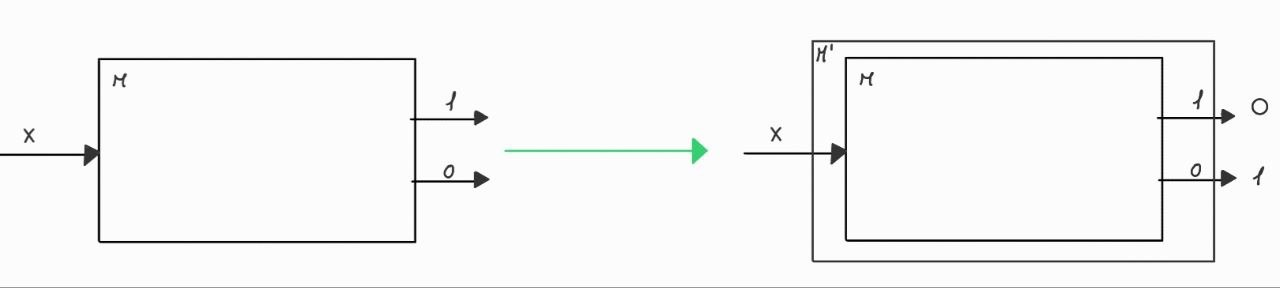
\includegraphics[width=0.5\textwidth]{img/MacchineTuring/dimostrazione1.png}
        \caption{Rappresentazione grafica della dimostrazione che il complemento
            di un linguaggio ricorsivo è ricorsivo}
    \end{figure}
\end{dimostrazione}
\begin{teorema}[\textbf{Linguaggio ricorsivo è anche ricorsivamente enumerabile}]
    Preso un linguaggio $L$ costruito alfabeto $\Sigma$ si ha che se
    $L \subseteq \Sigma^{\ast}$ se $L$ è ricorsivo è anche ricorsivamente
    enumerabile.
\end{teorema}
\begin{dimostrazione}
    Se $L$ è ricorsivo esiste una macchina di Turing che riconosce se, data una
    stringa $x$, tale che $x \in L$, rispondendo $1$ e risponde $0$ se $x \not\in
        L$.

    Costruisco ora una macchina di Turing $M'$ che se il linguaggio non è
    ricorsivo allora vado in loop ($\perp$). Quindi, quando la macchina sta per
    andare in $0$ modifico $\delta$ per ottenere il loop, ottenendo una macchina
    che va in loop se $x \not\in L$, mentre restituisce $1$ se $x \in L$ e
    quindi $L$ è ricorsivamente enumerabile.
    \begin{figure}[!ht]
        \centering
        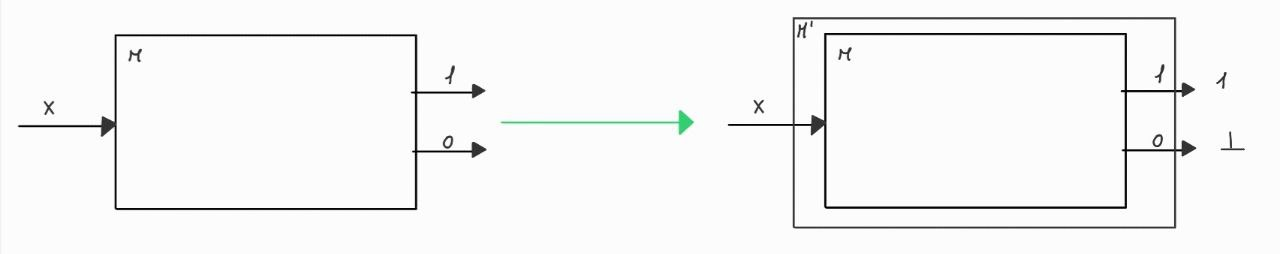
\includegraphics[width=0.5\textwidth]{img/MacchineTuring/dimostrazione2.png}
        \caption{Rappresentazione grafica della dimostrazione che un linguaggio
            ricorsivo è anche ricorsivamente enumerabile}
    \end{figure}
\end{dimostrazione}
\begin{teorema} \label{teo-rec-en-comp}
    $L$ è ricorsivo se e solo se $L$ è ricorsivamente enumerabile e il
    complementare di $L$, ossia $\overline{L}$, è ricorsivamente enumerabile.
\end{teorema}
\begin{dimostrazione}
    Rispetto alla dimostrazione precedente, che garantisce che se $L$ è ricorsivo
    allora è ricorsivamente enumerabile, devo definire, per il complementare,
    una macchina di Turing che va in loop se $x \in L$. Presa quindi una macchina
    di Turing $M$ che decide $L$, definisco $M'$ che accetta $L$, che quindi è
    ricorsivamente enumerabile. Definisco ora $M''$ che restituisce $1$ se
    $x \in \overline{L}$ ovvero $x \not\in L$ ed entra in loop se $x \not\in
        \overline{L}$, ovvero $x \in L$.

    Quindi $M$ decide $L$ eseguendo alternativamente $M'$ e $M''$ prestando
    attenzione alla gestione degli output.
\end{dimostrazione}
Vogliamo ora dimostrare che esistono dei problemi di decisione che non possono
essere risolti da una macchina di Turing. Per realizzare questa dimostrazione
partiamo dal fatto che $|A| < |\mathcal{P}(A)|$, ovvero che la cardinalità
dell'insieme $A$ è sempre minore della cardinalità dell'insieme delle parti di
$A$ ($\mathcal{P}(A)$).

Con le informazioni ottenute in precedenza abbiamo visto che possiamo
rappresentare una macchina di Turing partendo dall'alfabeto binario definito
come $B = \{0, 1\}$. Da questo, possiamo affermare che il numero di macchine di
Turing che possiamo realizzare sarà al più il numero di stringhe realizzabili
con l'utilizzo di $B$, ovvero $|B^{\ast}|$:
\begin{equation}
    |M| = |B^{\ast}|
\end{equation}
Inoltre, utilizzando l'alfabeto $B$, possiamo definire il linguaggio di
decisione come:
\begin{equation}
    L_D = \{x \in B^{\ast} \ | \ f_D(x) = 1\} \subseteq B^{\ast}
\end{equation}
quindi, possiamo affermare che il numero di problemi di decisione che si possono
avere è uguale a $|P(B^{\ast})|$. Partendo dal concetto matematico prima
presentato, possiamo affermare che:
\begin{equation}
    |M| = |B^{\ast}| < |P(B^{\ast})|
\end{equation}
ovvero che esistono problemi di decisione che \textit{non posso} risolvere con
una macchina di Turing.
\subsection{Halting Problem}
Un esempio di problema di decisione che non può essere risolto da una macchina
di Turing è l'\textbf{halting problem}. Questo problema consiste nel determinare
se esiste un algoritmo che dati in input una macchina di Turing $M$ e una stringa
$x$, mi dica se la macchina $M$ eseguita sull'input $x$ termina.
\begin{definizione}
    Posso definire formalmente l'\textbf{halting problem} con l'utilizzo del
    linguaggio $L_H$, definito come:
    \begin{equation}
        L_H = \{M \cdot \# \cdot x \ | \ M(x) \neq \perp \}
    \end{equation}
    ovvero come l'insieme di stringhe composte dalla descrizione di una macchina
    di Turing a cui è concatenato l'input tali per cui $M$ eseguita sull'input
    $x$ termina. Si utilizza il carattere $\#$ per separare la descrizione della
    macchina e l'input.
\end{definizione}
\begin{teorema}[\textbf{Halting problem non è decidibile}]
    Il linguaggio $L_H$ non è ricorsivo e quindi l'halting problem non è
    decidibile.
\end{teorema}
\begin{dimostrazione} [\textit{Per assurdo}]
    Assumiamo, per assurdo, che $L_H$ sia ricorsivo. Quindi esiste una macchina
    di Turing $M_H$ che prende in input $(M \cdot \# \cdot x)$ e mi fornisce in
    output:
    \begin{equation}
        M_H (M \cdot \# \cdot x) = \begin{cases}
            Y & \text{se} \ M(x) \ \neq \ \perp \\
            N & \text{se} \ M(x) \  = \ \perp
        \end{cases}
    \end{equation}
    Se esiste tale macchina, allora posso costruire una macchina di Turing $C$,
    costruita partendo da $M_H$ che prende in input $M$ e mi restituisce:
    \begin{equation}
        C(M) = \begin{cases}
            Y & \text{se} \ M_H(M, M) = N \\
            N & \text{se} \ M_H(M, M) = Y
        \end{cases}
    \end{equation}
    A questo punto se fornisco alla macchina $C$ se stessa come input ottenendo
    due possibili situazioni:
    \begin{itemize}
        \item $C(C) = Y$ allora $M_H(C, C) = N$ ma quindi mi aspetto che
              $C(C) = \perp$ il che mi porta ad un assurdo.
        \item $C(C) = \perp$ allora $M_H(C, C) =  Y$ ma quindi mi aspetto che
              $C(C) \neq \perp$ il che mi porta ad un assurdo.
    \end{itemize}
    Posso quindi affermare che non esiste una macchina $M_H$ che decide $L_H$.
    \begin{figure}[!ht]
        \centering
        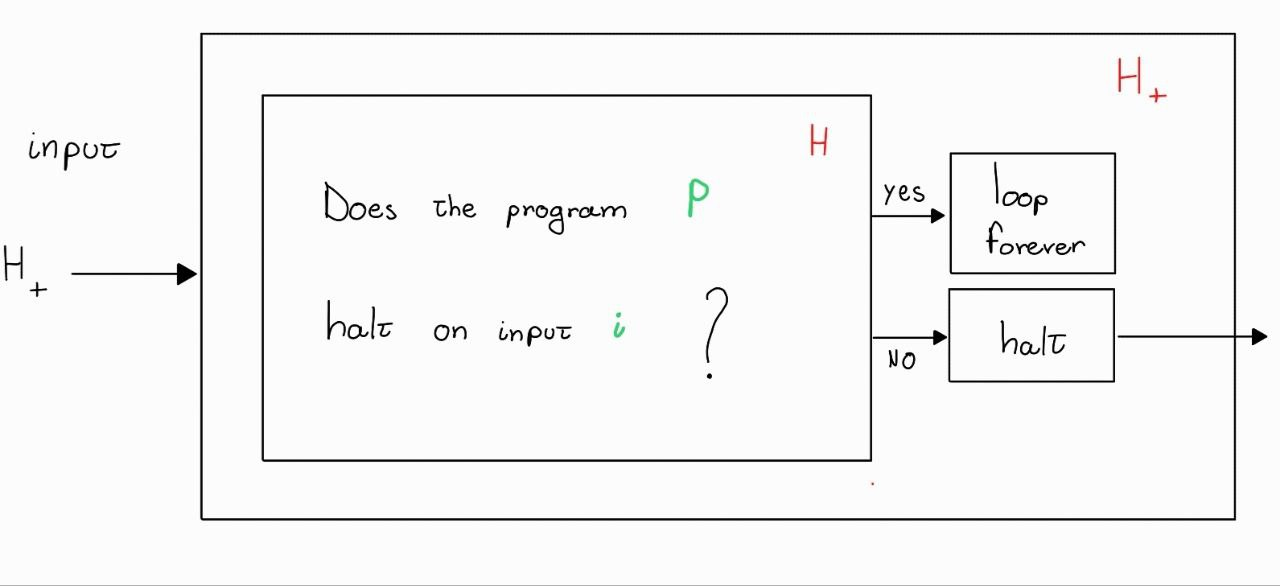
\includegraphics[width=0.5\textwidth]{img/MacchineTuring/halt.png}
        \caption{Rappresentazione grafica della dimostrazione dell'Halting problem}
    \end{figure}
\end{dimostrazione}
\begin{teorema}[\textbf{Halting problem è ricorsivamente enumerabile}] \label{teo-lh-rec-en}
    Il linguaggio $L_H$ è ricorsivamente enumerabile, ovvero il problema è
    parzialmente decidibile.
\end{teorema}
\begin{dimostrazione}
    Esiste una macchina di Turing $M_A$ che accetta il linguaggio $L_H$, ovvero
    tale che $M_A(M, x) = Y$ se e solo se $M(x) \neq \ \perp$.

    In precedenza abbiamo definito la macchina di Turing universale, la quale
    $U(M, x) = M(x)$, allora:
    \begin{equation}
        M_A(M, x) = \begin{cases}
            Y     & \text{se e solo se} \ U(M, x) = Y \ \lor \ N \\
            \perp & \text{se} \ U(M, x) = \perp
        \end{cases}
    \end{equation}
    Esiste quindi una macchina che accetta il linguaggio $L_H$.
\end{dimostrazione}
\begin{teorema}
    $\overline{L_H}$ non è ricorsivamente enumerabile.
\end{teorema}
\begin{dimostrazione} [\textit{Per assurdo}]
    Assumiamo per assurdo che $\overline{L_H}$ sia ricorsivamente enumerabile.
    Dal teorema \ref{teo-lh-rec-en} sappiamo che $L_H$ è ricorsivamente
    enumerabile, allora per quanto definito nel teorema \ref{teo-rec-en-comp} si
    ha che $L_H$ è ricorsivo, il che è assurdo in quanto è stato dimostrato che
    $L_H$ non è ricorsivo.
\end{dimostrazione}
\section{Problemi decidibili}
Vogliamo ora studiare i problemi decidibili classificandoli sulla base dei tempi
di esecuzione, considerando la dimensione dell'input e il caso peggiore. Per fare
questo utilizzeremo il tempo di esecuzione di una macchina di Turing. Questo
valore viene calcolato tramite il numero di passi che la macchina compie.
\begin{definizione}[\textbf{Tempo di calcolo}]
    Definiamo $t_M(x)$ come il tempo di calcolo di una macchina di Turing $M$ su
    input $x$. Non è il caso peggiore, ma dipendente dal singolo input specifico.
    Il tempo di calcolo è il numero di passi che esegue $M$ su input $x$ per
    dare una risposta.
\end{definizione}
Non si usa comunque il numero di passi nella realtà ma si usa la notazione
$\mathcal{O}$-grande, studiando il caso peggiore, ovvero il numero massimo di
passi.
\begin{definizione}[\textbf{Complessità temporale}]
    Definiamo $T_M(n)$ come la \textbf{funzione di complessità temporale} come:
    \begin{equation}
        T_M(n) = \max \{t_M(x) \ | \ |x| = n\}
    \end{equation}
\end{definizione}
\begin{definizione}[\textbf{Classe P}]
    Definisco la classe $P$ in base alle macchine di Turing. La classe $P$ è
    definita come:
    \begin{equation}
        P = \{L \ | \ L \ \text{ è deciso da una macchina di Turing in tempo }
        \mathcal{O}(p(n))\}
    \end{equation}
\end{definizione}
\begin{definizione}[\textbf{Classe DTIME}]
    Definiamo la classe $DTIME(f(n))$ come la classe dei linguaggi decisi da una
    macchina di Turing entro un tempo $f(n)$:
    \begin{equation}
        DTIME(f(n)) = \{L \subseteq \Sigma^{\ast} \ | \ \exists M \
        \text{decide} \ L \ \text{in tempo} \ \mathcal{O}(f(n)) \}
    \end{equation}
    Quindi $DTIME(n)$ rappresenta l'insieme dei problemi di decisione che possono
    essere risolti con un algoritmo che lavora in tempo $\mathcal{O}(n)$. Quindi:
    \begin{equation}
        P = \bigcup_{c \ \in \ \mathbb{N}} DTIME(n^c)
    \end{equation}
    Infatti $P$ è l'unione di tutte le classi DTIME con funzioni polinomiali.
\end{definizione}
Possiamo dire che vale la seguente relazione tra le classi $DTIME$:
\begin{equation}
    DTIME(n) \subseteq DTIME(n^2) \subseteq DTIME(2^{n^c})
\end{equation}
Possiamo anche definire la classe \textbf{EXPTIME} come la classe di linguaggi
decidibili da una macchina di Turing in tempo esponenziale:
\begin{equation}
    EXPTIME =  \bigcup_{c \ \in \ \mathbb{N}} DTIME(2^{n^c})
\end{equation}
Inoltre, si ha che vale la seguente relazione tra le classi $P$ e $EXPTIME$:
\begin{equation}
    P \subseteq EXPTIME
\end{equation}
\begin{teorema}
    Se un problema è nella classe $P$ allora è risolvibile in un tempo efficiente.
\end{teorema}
Devo anche definire la complessità spaziale oltre a quella temporale.
\begin{definizione}[\textbf{Spazio}]
    Definisco lo \textbf{spazio} di calcolo $s_M(x)$ come il numero di celle del
    nastro usate dalla macchina di Turing $M$ con input $x$ durante la
    computazione.

    Il calcolo non è semplice come per il tempo, avendo anche decrementi. Quindi
    più che “celle usate” studiamo le “celle visitate”.
\end{definizione}
\begin{definizione}[\textbf{Complessità spaziale}]
    Definisco $S_M(n)$ come la \textbf{funzione di complessità spaziale}:
    \begin{equation}
        S_M(n) =  \max\{s_M(x) \ | \ |x| = n\}
    \end{equation}
\end{definizione}
Esiste una relazione tra la complessità spaziale e quella temporale per una
macchina di Turing. Se una computazione dura $n$ passi di tempo, allora posso
dire che al più ho usato $n$ celle di spazio, questo perché è possibile che in
alcune configurazioni la testina non si muove, ma nel caso peggiore si sposta
sempre. Si ha quindi:
\begin{equation}
    S_M(n) \leq T_M(n) + n
\end{equation}
con $+ \ n$ perché sul nastro abbiamo comunque l'input di lunghezza $n$.
\begin{teorema}
    Se il tempo è limitato allora lo spazio è limitato ma non vale l'opposto.
\end{teorema}
\begin{teorema}
    Se ho una macchina di Turing $M$ che lavora in spazio finito e tempo infinito,
    esiste una macchina di Turing $M'$ che fa la stessa cosa di $M$ in tempo
    limitato. Quindi se lo spazio è limitato allora il tempo è limitato.
\end{teorema}
\begin{dimostrazione}
    Infatti la macchina $M'$ può trovarsi in un numero finito di stati $K$ e
    avendo spazio limitato ho un numero limitato $S_M(n)$ di celle in cui si trova
    la testina. Ho anche un numero finito di simboli in alfabeto $\Sigma$ e quindi:
    \begin{equation}
        S_{M'}(n) \leq |k| \cdot |S_M(n)| \cdot |\Sigma|^{|S_M(n)|}
    \end{equation}
    avendo che prima o poi ritorno a stati già visti quindi la macchina se supera
    la quantità appena definita capisce di essere in loop. Quindi
    $|k| \cdot |S_M(n)| \cdot |\Sigma|^{|S_M(n)|}$ è anche un limite temporale
    per la seconda macchina.
\end{dimostrazione}
Quindi data una certa macchina che lavora in un certo spazio $S(n)$ posso costruire
una macchina equivalente che da la stessa risposta in tempo limitato $T(n)$. Si ha
che se ho un problema che si risolve in spazio polinomiale, per la formula appena
scritta avrò tempo esponenziale. Invece, al contrario, tempo polinomiale comporta
spazio polinomiale.
\section{Macchine di Turing non deterministiche}
Una \textbf{macchina di Turing non deterministica} si distingue da quella
deterministica nella funzione di transizione $\delta$. Nella macchina non
deterministica la funzione di transizione associa a ogni stato $q$ e a ogni
simbolo di nastro $X$ un \textit{insieme} di triple:
\begin{equation}
    \delta(q, X) = \{(q_1, Y_1, D_1), (q_2, Y_2, D_2), \dots, (q_k, Y_k, D_k)\}
\end{equation}
A ogni passo una macchina di Turing non deterministica sceglie una delle triple
come mossa, ovviamente lo stato, il simbolo di nastro e la direzione appartengono
alla stessa tripla. Nelle macchine non deterministiche la computazione non è una
sequenza di configurazioni ma un albero di computazione. Da ogni stato posso
passare a uno tra più stati, a seconda della scelta, formando così un albero. Il
singolo passo di computazione non è univocamente definito. Ogni singolo ramo
comunque è equivalente al passo di computazione della macchina di Turing
deterministica.
\begin{definizione}[\textbf{Linguaggio accettato}]
    Un linguaggio $L$ è \textbf{accettato} da una macchina di Turing non
    deterministica $N$ se per tutte le stringhe che fanno parte del linguaggio
    esiste almeno una computazione che termina nello stato $Y$, ovvero esiste
    una computazione per cui:
    \begin{equation}
        \forall x \in L \Rightarrow N(x) = Y
    \end{equation}
    Nel caso in cui nessuna delle computazioni termina nello stato $Y$, allora
    l'input non è accettato.
\end{definizione}
\begin{definizione}[\textbf{Linguaggio deciso}]
    Un linguaggio $L$ è \textbf{deciso} da una macchina di Turing non
    deterministica $N$ se, qualora la stringa $x$ appartenga il linguaggio,
    esiste almeno una computazione tale per cui:
    \begin{equation}
        x \in L \to N(x) = Y
    \end{equation}
    altrimenti, se $x$ non appartiene al linguaggio (\textbf{rifiuta}), per
    tutte le computazioni, si ha che:
    \begin{equation}
        x \not\in L \to N(x) = N
    \end{equation}
    Non devo quindi avere loop in questo caso, tutte devono dare $N$.
\end{definizione}
\begin{teorema}[\textbf{Equivalenza tra macchine di Turing deterministica e non
            deterministica}]
    Se $M_N$ è una macchina di Turing non deterministica, esiste una macchina di
    Turing deterministica $M_D$ tale che accettano gli stessi linguaggi $L(M_N)
        = L(M_D)$.
\end{teorema}
\begin{dimostrazione}
    La macchina di Turing deterministica $M_D$ può simulare la macchina di Turing
    non deterministica $M_N$ procedendo con una visita in ampiezza dell'albero
    di computazione. Viene eseguita una visita in ampiezza in modo da evitare di
    incappare in loop.
\end{dimostrazione}
La macchina di Turing non deterministica $N$ decide il linguaggio $L$ in tempo
$t_N(n)$, ovvero il tempo di calcolo è dato dall'altezza del ramo più lungo.
Come per le macchine deterministiche, definiamo $T_N(n)$ come:
\begin{equation}
    T_N(n) = \max \{t_N(x) \ | \ |x| = n\}
\end{equation}
Data una macchina di Turing non deterministica $N$ che decide $L$ in tempo
$T_N(n)$ esiste una macchina di Turing deterministica $M$ che decide $L$ in tempo
$2^{\mathcal{O}(T_N(n))}$. Questa complessità deriva dal fatto che se ogni nodo
dell'albero ha al massimo $b$ figli, allora l'albero di computazione ha al
massimo $b^{T_N(n)}$ foglie. Il numero interno di nodi è al massimo $b^{T_N(n)}
    - 1$ e quindi il numero totale di nodi è $< 2 \cdot b^{T_N(n)}$. Inoltre, un
cammino dalla radice alla foglia è $\mathcal{O}(T_N(n))$. Il tempo di esecuzione
della macchina $M$ è:
\begin{equation}
    \mathcal{O}(T(n) \cdot b^{T(n)}) = 2^{\mathcal{O}(T_N(n))}
\end{equation}
\begin{definizione}[\textbf{Classe NTIME}]
    Definiamo una funzione di tempo per una macchina di Turing non deterministica
    come:
    \begin{equation}
        NTIME(f(n)) = \{L \ | \ L \ \text{è deciso da una macchina di Turing non
            deterministica in tempo } \mathcal{O}(f(n))\}
    \end{equation}
\end{definizione}
Quest'ultima definizione ci permette di definire la classe di \textbf{problemi NP}
come l'insieme dei linguaggi $L$ che sono decisi in tempo polinomiale da una
macchina di Turing non deterministica:
\begin{equation}
    NP = \bigcup_{c \in \mathbb{N}} NTIME(n^c)
\end{equation}
\begin{osservazione}
    Sia $P$ l'insieme dei \textbf{problemi decidibili in tempo polinomiale} da
    una macchina di Turing deterministica, e $NP$ l'insieme dei \textbf{problemi
        decidibili in tempo polinomiale} da una macchina di Turing non
    deterministica. Sappiamo che è vero che $P \subseteq NP$ ma non è ancora
    dimostrato che $NP \subseteq P$.
\end{osservazione}
Possiamo però affermare che:
\begin{equation}
    P \subseteq NP \subseteq EXPTIME
\end{equation}
\subsection{Verificatori}
La classe $NP$ rappresenta una classe di linguaggi che sono verificabili in
tempo polinomiale da una macchina di Turing non deterministica. Verificare un
linguaggio significa che per ogni input $x \in L$ si ha una stringa $c$ detta
\textbf{certificato} che possiamo usare per verificare che effettivamente $x \in
    L$.
\begin{definizione}[\textbf{Verificatore}]
    Un \textbf{verificatore} di un linguaggio $L$ è una macchina di Turing
    deterministica $V$ tale per cui:
    \begin{equation}
        L = \{x | V \ \text{accetta} \ \langle x, c \rangle \
        \text{per qualunque stringa} \ c\}
    \end{equation}
    Questa macchina accetta le stringhe appartenenti al linguaggio eseguendo le
    istruzioni specificate dal certificato $c$.
\end{definizione}
Se $V$ richiede tempo polinomiale rispetto $x$ a per accettare/rifiutare, allora
$V$ è un verificatore in tempo polinomiale per $x$. Se esiste un verificatore in
tempo polinomiale per $L$, allora $L$ è verificabile in tempo polinomiale.

Dato che $V$ deve eseguire in tempo polinomiale rispetto a $x$, ne segue che $c$,
il certificato, deve essere di lunghezza polinomiale rispetto a $x$, altrimenti
non avremmo il tempo di leggere tutto $c$.

Supponiamo di avere una macchina di Turing non deterministica $M$ che lavora in
tempo polinomiale, costruiamo un verificatore $V$ che lavora in tempo polinomiale
per lo stesso linguaggio deciso da $M$. Se su input $x$ la macchina $M$ accetta,
significa che esiste una computazione accettante $C_1, \dots, C_k$ di lunghezza
polinomiale rispetto a $x$. Per ogni passaggio da $C_i$ a $C_{i + 1}$ è stata
applicata una transizione definita dalla funzione di transizione di $M$.

Usiamo come certificato $c$ la sequenza di transizioni applicate lungo tutta la
computazione, le quali sono in numero polinomiale. Queste transizioni ci
identificano una specifica computazione della macchina di Turing non
deterministica $M$. Il verificatore deve solo simulare quella computazione, senza
fare scelte non deterministiche, dato che le transizioni da fare sono tutte in
$c$ e verificare che la computazione accetti.

Abbiamo mostrato che per ogni linguaggio accettato da una macchina di Turing non
deterministica che lavora in tempo polinomiale possiamo costruire un verificatore
polinomiale per lo stesso linguaggio.

Dobbiamo mostrare ora l'inclusione in senso inverso. Sfruttiamo il fatto che
possiamo usare una macchina di Turing non deterministica per scrivere un
certificato sul nastro e, se esiste un certificato che ci permette di accettare,
questo sarà presente in una computazione.

Sia $V$ un verificatore in tempo polinomiale per $L$. Assumiamo $V$ esegua in
tempo $n^k$. Costruiamo una macchina di Turing non deterministica che su input
$x$ esegue due compiti:
\begin{itemize}
    \item Genera in modo non deterministico un certificato $c$ di lunghezza al
          più $n^k$.
    \item Simula $V$ su input $\langle x, c \rangle$ e accetta se $V$ accetta,
          mentre rifiuta se $V$ rifiuta.
\end{itemize}
Abbiamo mostrato che per ogni linguaggio per il quale esiste un verificatore
polinomiale possiamo costruire una macchina di Turing non deterministica che
decide lo stesso linguaggio in tempo polinomiale. Quindi le due definizioni di
$NP$ sono equivalenti.
\begin{esempio}
    Consideriamo il problema del cammino Hamiltonian. Tale problema consiste nel
    dato un grafo orientato $G = (V, E)$ trovare trovare un cammino che visita
    tutti i nodi una sola volta. Consideriamo una variante in cui conosciamo il
    nodo di partenza $s$ e il nodo di arrivo $t$.
    \begin{equation}
        HAMPATH = \{\langle G, s, t \rangle \ | \ G \ \text{ha un cammino
            Hamiltonian da} \ s \ \text{a} \ t\}
    \end{equation}
    Per questo problema si può ottenere una semplice soluzione che lo risolve in
    tempo esponenziale, ovvero provare tutti i possibili cammini. Questa
    soluzione è però inefficiente.

    Questo problema ha una caratteristica chiamata \textit{verificabilità
        polinomiale}. Se in qualche modo si riesce a trovare un cammino
    Hamiltonian, allora possiamo verificare l'esistenza di tale cammino in tempo
    polinomiale.

    Per il problema del cammino Hamiltonian il certificato è rappresentato da
    un percorso Hamiltonian da $s$ a $t$. Il verificatore $V$ prende in input
    $\langle G, s, t, c \rangle$ e controlla che $c$ sia un cammino Hamiltonian
    da $s$ a $t$ in $G$. Per fare questo, il verificatore controlla che il primo
    nodo di $c$ sia $s$, che l'ultimo nodo sia $t$ e che ogni nodo di $c$ sia
    connesso al successivo.
    Da questo segue che il verificatore $V$ lavora in tempo polinomiale rispetto
    alla lunghezza del certificato $c$.
\end{esempio}
\subsection{Classi di problemi}
Definiamo ora altre classi di problemi:
\begin{itemize}
    \item \textbf{coP}: ovvero la classe di linguaggi di cui posso decidere la
          \textbf{non appartenenza} in tempo polinomiale:
          \begin{equation}
              coP = \{L \ | \ \overline{L} \in P\}
          \end{equation}
    \item \textbf{$\overline{P}$}: ovvero la classe di linguaggi che \textbf{non
              sono decidibili} in tempo polinomiale:
          \begin{equation}
              \overline{P} = \{L \ | \ L \not\in P\}
          \end{equation}
    \item \textbf{coNP}: ovvero la classe di linguaggi di cui posso decidere la
          \textbf{non appartenenza} in tempo polinomiale da una macchina di
          Turing non deterministica:
          \begin{equation}
              coNP = \{L \ | \ \overline{L} \in NP\}
          \end{equation}
\end{itemize}
\begin{nota}
    È importante notare che:
    \begin{equation}
        \overline{P} \neq coP
    \end{equation}
    \begin{equation}
        P \subseteq NP \ \land \ P \subseteq coNP \ \text{quindi} \ P
        \subseteq NP \cap coNP
    \end{equation}
\end{nota}
\begin{teorema}
    \begin{equation}
        P = coP
    \end{equation}
\end{teorema}
\begin{dimostrazione}
    Se un linguaggio $L \in P$, allora esiste una macchina di Turing
    deterministica che decide $L$ in tempo polinomiale:
    \begin{equation}
        \forall x \in \Sigma^{\ast} = \begin{cases}
            x \in L \Rightarrow M(x) = Y \\
            x \not\in L \Rightarrow M(x) = N
        \end{cases}
    \end{equation}
    Posso inoltre creare una macchina $M'$ che decide $\overline{L}$ in tempo
    polinomiale:
    \begin{equation}
        \forall x \in \Sigma^{\ast} = \begin{cases}
            x \in \overline{L} \Rightarrow M'(x) = Y \\
            x \not\in \overline{L} \Rightarrow M'(x) = N
        \end{cases}
    \end{equation}
    per ottenere questa macchina è sufficiente modificare gli stati di
    accettazione e rifiuto della macchina $M$.
\end{dimostrazione}
La dimostrazione precedente non può essere utilizzata per dimostrare che $NP =
    coNP$ dato che, nel caso di macchine non deterministiche è sufficiente che
esista un singolo ramo di computazione che termina in uno stato di accettazione.
Invertendo l'output di questa macchina si ottiene una macchina che non decide
$\bar{L}$ dato che sarebbero necessaire tutte computazioni che terminano in uno
stato accettante.
\section{Riduzioni polinomiali}
Le \textbf{riduzioni polinomiali} tra problemi sono delle procedure che per ogni
istanza del problema $A$ la trasformano in un'istanza per un problema diverso $B$.
Quindi un'istanza di $A$, $I_A$, ha due risposte, $Y$ o $N$, ma posso passare
tramite una determinata funzione $f$, definita come:
\begin{equation}
    f: I_A \to I_B
\end{equation}
a un istanza $I_B$ tale che $B$ avrà risposte, uguali a quelle di $A$, $Y$ o $N$.
\begin{equation}
    \forall x \in I_A \ \begin{cases}
        A(x) = Y \Rightarrow B(f(x)) = Y \\
        A(x) = N \Rightarrow B(f(x)) = N
    \end{cases}
\end{equation}
In altre parole, si cerca una funzione $f$ che mi permette di convertire le
istanze del mio problema di partenza in istanze di un problema che so risolvere.
\begin{definizione}[\textbf{Riduzione polinomiale}]
    La \textbf{riducibilità polinomiale} tra problemi è definita come:
    \begin{equation}
        f: \Sigma^{\ast} \to \Sigma^{\ast}
    \end{equation}
    la quale deve essere calcolabile in tempo polinomiale da una macchina di
    Turing deterministica, tale che:
    \begin{equation}
        \forall x \in \Sigma^{\ast}, \ x \in L_A \ \text{se e solo se} \
        f(x) \in L_B
    \end{equation}
    Indichiamo l'operazione di riduzione polinomiale come:
    \begin{equation}
        L_A \leq_P L_B
    \end{equation}
\end{definizione}
\begin{osservazione}
    Si utilizza il simbolo minore uguale ($\leq$), per indicare una relazione
    d'ordine nella complessità dei problemi.
\end{osservazione}
\begin{teorema}
    Dato un linguaggio $L_A$ riducibile polinomialmente a $L_B$ ($L_A \leq_P L_B$),
    si ha che se $L_B \in P$ allora sicuramente anche $L_A \in P$.
\end{teorema}
\begin{dimostrazione}
    Infatti e esiste un algoritmo polinomiale per $L_B$ allora, avendo una
    trasformazione polinomiale ho che $f(x) + L_B$ è ancora polinomiale.
\end{dimostrazione}
\begin{teorema}[\textbf{Transitività}]
    La riduzione polinomiale gode della proprietà di transitività, ovvero:
    \begin{equation}
        L_A \ \leq_P \ L_B \ \land \ L_B \ \leq_P \ L_C \ \text{allora} \ L_A
        \ \leq_P \ L_C
    \end{equation}
    Posso ottenere questa riduzione applicando la composizione di funzioni.
\end{teorema}
\begin{definizione}[\textbf{NP-hard}]
    Un linguaggio $L$ è \textbf{NP}$\_$\textbf{hard} se vale che:
    \begin{equation}
        \forall L' \in NP \ \text{si ha} \ L' \leq_P L
    \end{equation}
\end{definizione}
\begin{definizione}[\textbf{NP-completo}]
    Un linguaggio $L$ si dice \textbf{NP}$\_$\textbf{completo} se valgono i
    seguenti punti:
    \begin{itemize}
        \item $L \in NP$
        \item $L \in NP\_hard$
    \end{itemize}
\end{definizione}
\begin{teorema}
    Se $L_A \leq_P L_B$ e $L_A \in NP\_hard$ allora so che anche $L_B \in NP\_hard$.
\end{teorema}
\begin{dimostrazione}
    Se $L_A \leq_P L_B$ per la definizione di $NP\_hard$ so che esistono n
    linguaggi che sono riducibili polinomialmente a $L_A$. Utilizzando la
    proprietà transitiva posso affermare che $L_B$ è $NP\_hard$.
\end{dimostrazione}
\begin{teorema}[\textbf{Teorema Cook-Levin}]
    Il problema di soddisfacibilità SAT è \textbf{NP}$\_$\textbf{completo}.
    Questo problema prende in input una formula booleana $\phi$ in forma normale
    congiunta (CNF), ovvero che ha una congiunzione ($\land$) come legame tra le
    clausole. Una clausola è un $\lor$ di letterali, ovvero di variabili booleane
    $x_i$ o $\overline{x_i}$. In output ho se la forma sia soddisfacibile o meno.
\end{teorema}
\begin{figure}[!ht]
    \centering
    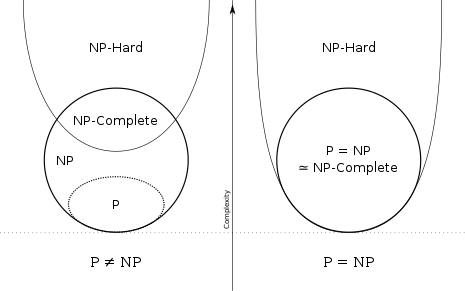
\includegraphics[width=0.5\textwidth]{img/MacchineTuring/classificazioneProblemi.png}
    \caption{Classificazione dei problemi.}
\end{figure}